\documentclass[11pt,a4paper]{article}
\usepackage[margin=2.5cm]{geometry}
\usepackage{amsmath,amssymb}
\usepackage{booktabs}
\usepackage{array}
\usepackage{xcolor}
\usepackage{tcolorbox}
\tcbuselibrary{skins,breakable}
\usepackage{hyperref}
\usepackage[numbers,sort&compress]{natbib}
\bibliographystyle{unsrtnat}
\hypersetup{colorlinks=true,linkcolor=blue!60!black,urlcolor=blue!60!black}
\setlength{\emergencystretch}{2em}
\usepackage{tikz}
\usetikzlibrary{arrows.meta,positioning,shapes.geometric}
\usepackage{enumitem}

\definecolor{boxblue}{RGB}{220,235,255}
\definecolor{boxorange}{RGB}{255,240,210}
\definecolor{boxgreen}{RGB}{220,245,220}
\definecolor{boxgold}{RGB}{255,248,210}
\definecolor{boxpurple}{RGB}{238,230,255}

\newcommand{\term}[1]{\textbf{#1}}
\newcommand{\poly}{p}
\newcommand{\Nfam}{N_{\mathrm{fam}}}
\newcommand{\lean}[1]{\texttt{#1}}

\title{\textbf{The Master Quadratic: One Equation, Two Crown Jewels}\\[6pt]
\large From the Diagonal of the GTE Polynomial to the Higgs Boson and Rule~110\\[4pt]
\normalsize\textit{UGP Physics Tutorial Series}
\\[2pt]\small\href{https://doi.org/\TutorialDOI}{doi.org/\TutorialDOI}}
\author{Nova Spivack\\[4pt]
\normalsize
\href{https://novaspivack.com/research}{novaspivack.com/research}
}
\newcommand{\TutorialDOI}{10.5281/zenodo.20657868}
\date{2026}

\begin{document}
\setcounter{tocdepth}{2}
\maketitle
\tableofcontents
\newpage

\begin{tcolorbox}[colback=blue!6,colframe=blue!40!black,
  title=\textbf{UGP Physics Tutorial Series}]
\textbf{Prerequisites (read first):} \href{https://doi.org/10.5281/zenodo.20657889}{\emph{The GTE Polynomial: A Step-by-Step Cheat Sheet}}\\[4pt]
\textbf{See also:} \href{https://doi.org/10.5281/zenodo.20657872}{\emph{The Levels of the Theory}} $\cdot$
\href{https://doi.org/10.5281/zenodo.20657876}{\emph{How MDL Selects the 19-Bit Polynomial}}
\end{tcolorbox}

\begin{tcolorbox}[colback=boxgreen,colframe=green!50!black,
  title=\textbf{Claim-Strength Taxonomy}]
Throughout this tutorial, results are labeled with a confidence grade:
\begin{itemize}[itemsep=2pt]
  \item \textbf{$\mathbf{A}_{\rm Lean}$ (CatAL)} --- Machine-certified in Lean~4 with zero \texttt{sorry} and zero custom axioms.  Independently verifiable by anyone with Lean installed.
  \item \textbf{A/D (CatAD)} --- Analytically derived with full derivation, computationally confirmed.  Not yet machine-certified.
  \item \textbf{A (CatA)} --- Analytically derived; derivation complete but not independently machine-certified.
  \item \textbf{A/D (conditional)} --- Derived under a named, stated premise; the premise is itself an open problem or a CatB assumption.
  \item \textbf{B (CatB)} --- A stated working hypothesis or structural premise; not yet derived.
\end{itemize}
\end{tcolorbox}

%─────────────────────────────────────────────────────────────────────────────
\section{The Diagonal: Setting \texorpdfstring{$L = C = R = x$}{L=C=R=x}}
%─────────────────────────────────────────────────────────────────────────────

\begin{tcolorbox}[colback=boxblue,colframe=blue!40!black,title=Key idea]
The polynomial $p$ normally takes three \emph{different} inputs.
What if all three are the same?
Setting $L = C = R = x$ reveals a hidden quadratic lurking inside
the 3-body rule — the ``master quadratic.''
\end{tcolorbox}

\subsection{What ``the diagonal'' means}

A cellular automaton is a row of cells, each with its own value.  The polynomial
$p(L,C,R)$ is built for the general case where Left, Centre, and Right all differ.
But we can ask a special question: what happens on a perfectly \emph{uniform}
configuration — one where every cell holds the same value $x$?

Mathematically, this means setting $L = C = R = x$ and evaluating $p(x,x,x)$.
This is called \term{evaluating on the diagonal} of the polynomial.

\subsection{Computing $p(x,x,x)$ step by step}

Substitute $L = C = R = x$ into $p(L,C,R) = C + R - CR - LCR$:

\begin{align*}
  p(x,x,x)
    &= x + x - x \cdot x - x \cdot x \cdot x \\
    &= 2x - x^2 - x^3.
\end{align*}

Nothing exotic: just algebra.  The result is a cubic in $x$.

\subsection{The self-consistency question}

A natural follow-up: for which values of $x$ does a uniform-$x$ configuration
\emph{stay} uniform?  Formally: when does $p(x,x,x) = x$?  Such a value is
called a \term{diagonal fixed point}.

Rearranging $p(x,x,x) = x$:
\[
  p(x,x,x) - x
  \;=\; 2x - x^2 - x^3 - x
  \;=\; x - x^2 - x^3
  \;=\; -x\bigl(x^2 + x - 1\bigr).
\]
So $p(x,x,x) = x$ if and only if $-x(x^2 + x - 1) = 0$, i.e.\ either
$x = 0$ or $x^2 + x - 1 = 0$.

\begin{tcolorbox}[colback=boxgreen,colframe=green!50!black,
  title=The universal diagonal factorization (machine-certified)]
Over any number system,
\[
  \boxed{p(x,x,x) - x \;=\; -\,x\,(x^2 + x - 1).}
\]
This identity is a universal algebraic fact, machine-certified in Lean~4
with zero sorry as \lean{gte\_diagonal\_quadratic\_factorization}.
The factor $m(x) = x^2 + x - 1$ is the \term{master quadratic}.
\end{tcolorbox}

The diagonal fixed-point equation has two families of solutions:
\begin{itemize}[itemsep=2pt]
  \item $x = 0$: the \emph{vacuum} — the all-zero configuration is always a fixed point.
  \item $m(x) = x^2 + x - 1 = 0$: solutions of the master quadratic (if any exist
    in the number system at hand).
\end{itemize}

How many solutions the master quadratic has — and in \emph{which} number systems —
governs two of the deepest results in the GTE framework.

%─────────────────────────────────────────────────────────────────────────────
\section{The Discriminant: \texorpdfstring{$\Delta = 5 = \Nfam$}{disc = 5 = N\_fam}}
%─────────────────────────────────────────────────────────────────────────────

\subsection{What is a discriminant?}

For a quadratic $ax^2 + bx + c$, the \term{discriminant} is
\[
  \Delta = b^2 - 4ac.
\]
It is the expression under the square root in the quadratic formula:
\[
  x = \frac{-b \pm \sqrt{\Delta}}{2a}.
\]
The discriminant determines whether the equation has solutions, and \emph{where}:
\begin{itemize}[itemsep=2pt]
  \item $\Delta > 0$: two distinct real roots.
  \item $\Delta = 0$: one repeated real root.
  \item $\Delta < 0$: no real roots (complex roots only).
  \item $\Delta$ is a quadratic non-residue mod $q$: no roots in the clock-arithmetic
    field $\mathrm{GF}(q)$.
\end{itemize}
The last case is central to Crown Jewel~2 in §\ref{sec:gf7}.

\subsection{Computing the discriminant of $x^2 + x - 1$}

For the master quadratic $m(x) = x^2 + x - 1$, we have $a = 1$, $b = 1$, $c = -1$:
\[
  \Delta
  = b^2 - 4ac
  = 1^2 - 4 \cdot 1 \cdot (-1)
  = 1 + 4
  = \mathbf{5}.
\]

\subsection{The structural identity: $\Delta = \Nfam = 5$}

In the GTE framework, $\Nfam = 5$ is the number of \term{fermion families} — the
five particle types in a single Standard Model generation: electron, up quark,
down quark, right-handed neutrino, left-handed neutrino.  This number is derived
independently from the $\mathbb{Z}_5$ orbit structure of the gauge sector (established
in P01~\cite{SpivackSM}), not inserted by hand.

The identity $\Delta = \Nfam = 5$ is structural: the family count is exactly the
discriminant of the polynomial's diagonal self-consistency core.  Every result that
flows from the master quadratic — the Higgs VEV, the binary computational floor,
vacuum uniqueness — inherits a link to the number of particle families.

\begin{tcolorbox}[colback=boxorange,colframe=orange!60!black,title=Summary so far]
\[
  p(x,x,x) - x = -x\,(x^2 + x - 1), \qquad \Delta = 5 = \Nfam.
\]
The master quadratic $x^2 + x - 1$ sits inside the diagonal of $p$.
Its discriminant equals the fermion family count.
Its behavior over $\mathbb{R}$ and over $\mathrm{GF}(7)$ are the two
``crown jewels'' of the framework.
\end{tcolorbox}

%─────────────────────────────────────────────────────────────────────────────
\section{Crown Jewel 1: The Golden Ratio and the Higgs VEV}
%─────────────────────────────────────────────────────────────────────────────

\begin{tcolorbox}[colback=boxgold,colframe=orange!70!black,
  title=Crown Jewel 1 — over $\mathbb{R}$]
Over the real numbers, $x^2 + x - 1 = 0$ has a positive root
$x^* = (\sqrt{5}-1)/2 = 1/\varphi$, the reciprocal of the golden ratio.
This is the SRRG fixed point — the self-consistent electroweak coupling —
that seeds the Higgs vacuum expectation value $v = 246.16\;\mathrm{GeV}$.
\end{tcolorbox}

\subsection{Computing the real roots}

Apply the quadratic formula to $x^2 + x - 1 = 0$ (so $a = 1$, $b = 1$, $c = -1$,
$\Delta = 5$):
\[
  x = \frac{-1 \pm \sqrt{5}}{2}.
\]

\begin{center}
\begin{tabular}{lcc}
\toprule
Root & Exact value & Approximation \\
\midrule
$x^+ = \dfrac{-1+\sqrt{5}}{2}$ & $= 1/\varphi$ & $\approx 0.6180$ \\[8pt]
$x^- = \dfrac{-1-\sqrt{5}}{2}$ & $= -\varphi$  & $\approx -1.6180$ \\
\bottomrule
\end{tabular}
\end{center}

\medskip
Here $\varphi = (1+\sqrt{5})/2 \approx 1.618$ is the \term{golden ratio}.
The positive root $x^+ = (\sqrt{5}-1)/2$ is exactly the reciprocal of the
golden ratio, $1/\varphi = \varphi - 1$.

\noindent\textit{Verification:} $(1/\varphi)^2 + (1/\varphi) - 1
  = (\varphi-1)^2 + (\varphi-1) - 1
  = \varphi^2 - 2\varphi + 1 + \varphi - 1 - 1
  = \varphi^2 - \varphi - 1 = 0$
(since $\varphi^2 = \varphi + 1$ by the golden ratio property). \checkmark

\subsection{The Self-Referential Renormalization Group}

The \term{Self-Referential Renormalization Group} (SRRG) asks: is there an
electroweak coupling $g$ that is \emph{self-consistent} with the universe's
own dynamics?  More precisely — in a universe whose fundamental rule is
$p$ — does there exist a coupling strength at which the dynamics, applied
to itself, reproduces that same coupling?

This is a fixed-point question.  Written in terms of the GTE polynomial,
the SRRG fixed-point equation is:
\[
  p(g, g, g) \;=\; g.
\]
From our computation, the non-trivial positive solution is:
\[
  g^* = \frac{\sqrt{5}-1}{2} = \frac{1}{\varphi} \approx 0.618.
\]
The golden ratio is not an \emph{assumption}; it is the \emph{output} of the
self-consistency equation of the master polynomial.  Plain English: the golden
ratio is the tuning fork that sets the electroweak scale — the unique
self-consistent frequency at which the universe's own algebra resonates.

The Lean certification \lean{gte\_poly\_srrg\_bridge} (zero sorry) establishes
that the SRRG fixed-point equation and the golden root of the master quadratic
are one and the same object.

\subsection{From the fixed point to the Higgs VEV}

The \term{Higgs vacuum expectation value} $v$ is the energy scale at which
electroweak symmetry is broken, giving the $W^\pm$ and $Z$ bosons their masses.
Experimentally, $v \approx 246.22$~GeV (derived from the Fermi constant $G_F$).

In the Standard Model, $v$ is a free parameter — it is fitted to data.  In GTE,
it is derived from the SRRG fixed point.  The fixed-point coupling
$g^* = 1/\varphi$, combined with the generation structure
($\Nfam = 5$ from the $\mathbb{Z}_5$ orbit), gives:
\[
  v_{\mathrm{PSC}} = 246.16\;\mathrm{GeV}
  \qquad \text{(GTE prediction, machine-certified in Lean~4)}.
\]
The route from $g^*$ to $v$ runs through the SRRG renormalization-group cascade:
the golden-ratio fixed point seeds the cascade, and the single dimensional anchor
$m_\tau = 1776.86$\,MeV combined with $\Nfam = 5$ sets the energy scale;
see P48 Chapter~7 for the explicit derivation.
The agreement is $246.16/246.22 \approx 99.976\%$: a $0.024\%$ discrepancy
with zero free parameters.

\begin{tcolorbox}[colback=boxgold,colframe=orange!70!black,
  title=Why the golden ratio?]
The golden ratio satisfies $\varphi = 1 + 1/\varphi$ — it is self-similar by
definition.  In GTE, the electroweak coupling satisfies the analogous
self-referential equation: $p(g,g,g) = g$.  These are the same equation in
disguise.  The golden ratio is the algebraic fingerprint of self-reference
in a universe governed by $p$.
\end{tcolorbox}

%─────────────────────────────────────────────────────────────────────────────
\section{Crown Jewel 2: Rootlessness over GF(7) and the Binary Floor}
\label{sec:gf7}
%─────────────────────────────────────────────────────────────────────────────

\begin{tcolorbox}[colback=boxpurple,colframe=blue!50!black,
  title=Crown Jewel 2 — over $\mathrm{GF}(7)$]
Over the integers mod~7, the equation $x^2 + x - 1 = 0$ has \emph{no} solution.
This rootlessness is the precise algebraic reason why the binary sector
$\{0,1\}$ is the \emph{unique} minimal invariant sub-automaton of $p$ — which
is why Rule~110, restricted to binary inputs, is computationally universal.
\end{tcolorbox}

\subsection{Quadratic residues and non-residues}

Recall from the Polynomial Cheat Sheet: in GF(7), all arithmetic is done
modulo~7.  Not every number has a square root in this finite world.

A \term{quadratic residue} mod~7 is a number that equals $k^2 \bmod 7$ for
some $k \in \{0, 1, \ldots, 6\}$.  A \term{quadratic non-residue} (QNR) is
a number that is \emph{not} the square of anything mod~7.

\subsection{The squares of GF(7): a worked calculation}

Compute $k^2 \bmod 7$ for every $k \in \{0, 1, 2, 3, 4, 5, 6\}$:

\bigskip
\begin{center}
\begin{tabular}{cccc}
\toprule
$k$ & $k^2$ (ordinary) & $k^2 \bmod 7$ & Remainder check \\
\midrule
0 & $0$  & $0$ & $0 = 7 \times 0 + 0$ \\
1 & $1$  & $1$ & $1 = 7 \times 0 + 1$ \\
2 & $4$  & $4$ & $4 = 7 \times 0 + 4$ \\
3 & $9$  & $2$ & $9 = 7 \times 1 + 2$ \\
4 & $16$ & $2$ & $16 = 7 \times 2 + 2$ \\
5 & $25$ & $4$ & $25 = 7 \times 3 + 4$ \\
6 & $36$ & $1$ & $36 = 7 \times 5 + 1$ \\
\bottomrule
\end{tabular}
\end{center}
\bigskip

The quadratic \emph{residues} mod~7 — the values that appear in the
``$k^2 \bmod 7$'' column — are $\{0, 1, 2, 4\}$.
The values $\{3, 5, 6\}$ never appear.  In particular:
\[
  5 \;\text{ is a quadratic non-residue mod } 7.
\]
This is a finite arithmetic fact, machine-certified as \lean{five\_is\_qnr\_mod7}
(Lean~4, zero sorry, proved by \texttt{decide}).

\subsection{Why 5 being a QNR means the quadratic has no root}

The quadratic formula gives roots $x = (-1 \pm \sqrt{5})/2$.  In GF(7),
computing $\sqrt{5}$ requires finding $s$ with $s^2 \equiv 5 \pmod 7$.  But
we just showed 5 is not among the squares mod~7 — so $\sqrt{5}$ does not
exist in GF(7).  The formula cannot produce a value, and the equation has
no solution.

We can also verify directly by checking all seven candidates:

\bigskip
\begin{center}
\begin{tabular}{ccl}
\toprule
$x$ & $x^2 + x - 1 \pmod 7$ & Is it $\equiv 0$? \\
\midrule
$0$ & $0 + 0 - 1 = -1 \equiv 6$      & No \\
$1$ & $1 + 1 - 1 = 1$                & No \\
$2$ & $4 + 2 - 1 = 5$                & No \\
$3$ & $9 + 3 - 1 = 11 \equiv 4$      & No \\
$4$ & $16 + 4 - 1 = 19 \equiv 5$     & No \\
$5$ & $25 + 5 - 1 = 29 \equiv 1$     & No \\
$6$ & $36 + 6 - 1 = 41 \equiv 6$     & No \\
\bottomrule
\end{tabular}
\end{center}
\bigskip

None of the seven elements of GF(7) satisfies $x^2 + x - 1 = 0$.
The master quadratic is \term{rootless} over GF(7).

\subsection{Why rootlessness forces the binary floor}

Return to the diagonal fixed-point equation: $p(x,x,x) = x$ has solutions
$x = 0$ (vacuum) or $x^2 + x - 1 = 0$ (master quadratic).  Over GF(7),
the master quadratic has no solutions.  Therefore the \emph{only} constant
diagonal fixed point of $p$ over GF(7) is $x = 0$ — the vacuum.

Now ask: could some non-binary value $k \in \{2, 3, 4, 5, 6\}$ ``anchor''
a non-trivial invariant sub-automaton — a smaller set of states that the
dynamics maps to itself, sitting between $\{0,1\}$ and the full 7-state system?
A necessary condition for $k$ to do so is that $p(k,k,k) = k$ (the constant-$k$
configuration must be fixed).  But the only constant fixed point is $k = 0$.
No non-binary value qualifies.

Conclusion: the smallest non-trivial invariant subset under $p$ in GF(7) is
exactly $\{0, 1\}$ — the \term{binary floor}.  The dynamics cannot produce
an intermediate sub-automaton anywhere between the vacuum and the full 7-state
system.

This is why Rule~110 is not merely \emph{a} binary restriction of $p$ but
the \emph{unique minimal computational layer}.  The rootlessness of
$x^2 + x - 1$ over GF(7) forces it.

\begin{tcolorbox}[colback=boxpurple,colframe=blue!50!black,
  title=Lean certifications]
The QNR uniqueness theorem — $\{0,1\}$ is the unique minimal invariant subset
of $p$ over GF(7) because $\Nfam = 5$ is a quadratic non-residue mod~7 — is
machine-certified in Lean~4 (zero sorry):
\begin{itemize}[itemsep=1pt]
  \item \lean{five\_is\_qnr\_mod7} — the arithmetic fact: 5 is not a square mod~7
  \item \lean{nfam\_qnr\_explains\_binary\_floor} — the structural implication
\end{itemize}
Module: \lean{UgpLean/Universality/Z7InvariantSubsets.lean}.

The rootlessness is also 7-adically robust: $x^2 + x - 1$ has no root
modulo $7^k$ for \emph{any} power $k \geq 1$, certified by\\
\mbox{\lean{master\_quadratic\_no\_root\_mod\_seven\_pow}}.
\end{tcolorbox}

\begin{tcolorbox}[colback=boxorange,colframe=orange!60!black,
  title=Complete invariant-subset taxonomy at \texorpdfstring{$q=7$}{q=7}]
The $p$-invariant subsets of $\mathrm{GF}(7)$ — sets $S$ such that
$p(x,y,z) \in S$ whenever $x,y,z \in S$ — are \emph{exactly}:
\begin{enumerate}[itemsep=2pt]
  \item $\{0\}$ — the vacuum point.
  \item $\{0,1\}$ — the binary floor; the unique non-trivial proper invariant subset.
  \item $\mathrm{GF}(7)$ itself — the full 7-state system.
\end{enumerate}
No proper subset of size $3, 4, 5,$ or $6$ is $p$-invariant.
The proof: any size-$\geq 3$ proper invariant set would require a non-binary
constant fixed point $k \neq 0$ (i.e.\ $p(k,k,k) = k$), but $k=0$ is the
unique constant fixed point (the master quadratic has no root over $\mathrm{GF}(7)$).
The general statement — for any prime $q$ where $x^2+x-1$ is rootless —
is that the only $p$-invariant subsets are $\{0\}$, $\{0,1\}$, and $\mathrm{GF}(q)$.
This is a complete characterization; the analytic proof for all rootless primes
is given in P49~\cite{SpivackGTEPolynomialWolfram}.
\end{tcolorbox}

%─────────────────────────────────────────────────────────────────────────────
\section{The All-$q$ Dichotomy Theorem}
\label{sec:dichotomy}
%─────────────────────────────────────────────────────────────────────────────

The rootlessness over GF(7) is not special to the prime~7.  The splitting
behaviour of $m(x) = x^2 + x - 1$ over $\mathrm{GF}(q)$ obeys a clean rule,
the \term{all-$q$ dichotomy theorem} (P49~\cite{SpivackGTEPolynomialWolfram}, Theorem~4.4):

\begin{tcolorbox}[colback=boxorange,colframe=orange!60!black,
  title=All-$q$ dichotomy]
For any prime $q \neq 2, 5$:
\[
  x^2 + x - 1 = 0 \text{ has roots in } \mathrm{GF}(q)
  \;\iff\;
  5 \text{ is a QR mod } q
  \;\iff\;
  q \equiv \pm 1 \pmod{5}.
\]
\textbf{Rootless (QNR) branch} ($q \equiv \pm 2 \pmod 5$, e.g.\ $q = 7, 13, 37, \ldots$):
$\{0,1\}$ is the unique binary floor; Rule~110 universality is forced.\\[4pt]
\textbf{Split (QR) branch} ($q \equiv \pm 1 \pmod 5$, e.g.\ $q = 11, 19, 29, \ldots$):
the quadratic has two roots; additional invariant subsets emerge.\\[4pt]
\textbf{Ramified case} ($q = 5$): discriminant vanishes, the quadratic is
$(x+3)^2$ with double root $x = 2$.  (This is the ``displaced vacuum'' pathology
of the GF(5) world.)
\end{tcolorbox}

The prime $q = 7$ satisfies $7 \equiv 2 \pmod{5}$, placing it firmly on the
rootless branch — the unique class of primes where $\Nfam = 5$ obstructs
any intermediate invariant sub-automaton.

\medskip
\begin{center}
\begin{tabular}{cccc}
\toprule
Prime $q$ & $q \bmod 5$ & 5 is\ldots & Master quadratic over GF($q$) \\
\midrule
2  & 2 & special    & Irreducible \\
5  & 0 & Ramified   & Double root $(x+3)^2$ \\
7  & 2 & \textbf{QNR} & \textbf{Rootless} $\leftarrow$ our universe \\
11 & 1 & QR         & Two distinct roots \\
13 & 3 & QNR        & Rootless \\
19 & 4 & QR         & Two distinct roots \\
29 & 4 & QR         & Two distinct roots \\
37 & 2 & QNR        & Rootless \\
\bottomrule
\end{tabular}
\end{center}

\medskip
The prime 7 is not chosen because it gives a nice result; it is determined
by independent constraints (the ridge minimality theorem of P01).  The QNR
condition is then verified as a \emph{consequence}.  The computational floor
is a theorem, not a design choice.

%─────────────────────────────────────────────────────────────────────────────
\section{One Quadratic, Two Scales}
\label{sec:unification}
%─────────────────────────────────────────────────────────────────────────────

\subsection{The unification}

The same $\mathbb{Z}$-polynomial $m(x) = x^2 + x - 1$ — discriminant $5 = \Nfam$ —
controls two previously separate derivation chains via its two natural arithmetic
completions:

\begin{itemize}
  \item \textbf{Over $\mathbb{R}$} (archimedean completion): the polynomial splits,
    yielding the golden root $1/\varphi$ that is the SRRG fixed point and seeds
    the Higgs VEV $v = 246.16$~GeV.
  \item \textbf{Over GF(7)} (7-adic completion): the polynomial is inert,
    with no roots — the mechanism that makes $\{0,1\}$ the unique binary floor
    and forces Rule~110 computational universality.
\end{itemize}

These are not two separate facts that happen to share a quadratic.  They are
both arithmetic images of the single integer polynomial $m$ under the
two completion maps $\mathbb{Z}[x] \to \mathbb{R}[x]$ and
$\mathbb{Z}[x] \to \mathrm{GF}(7)[x]$.  This unification is the
\emph{Golden-Quadratic Duality} theorem (P49 §3.2, CatAD; core components CatAL).

\subsection{Diagram}

\begin{center}
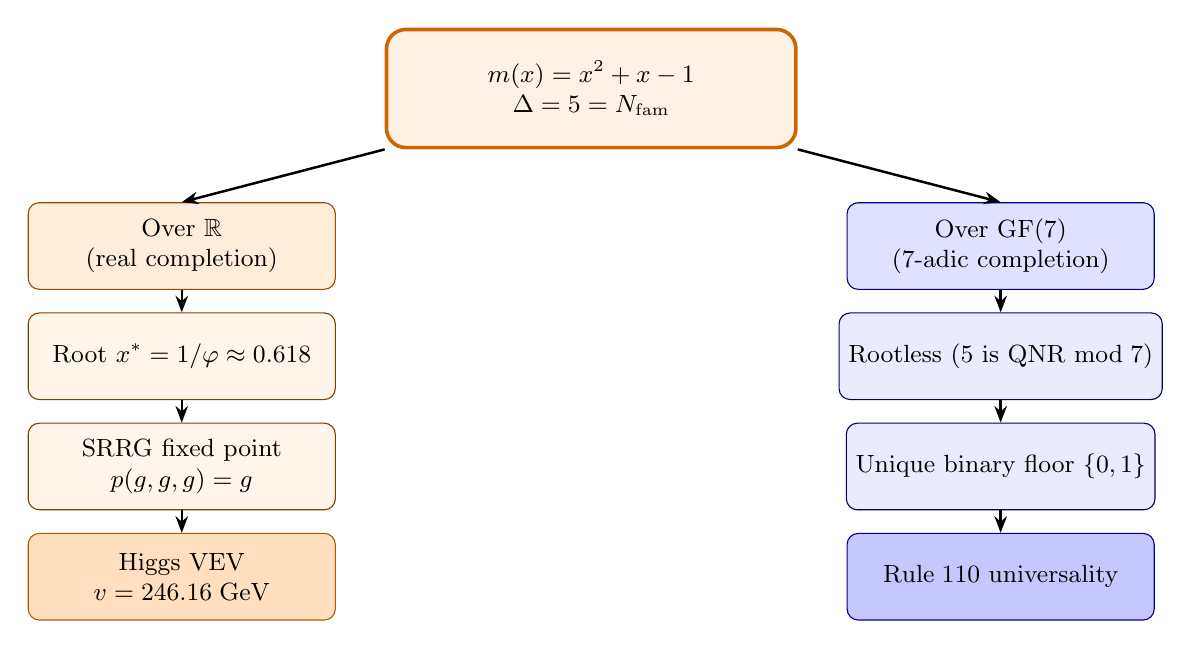
\begin{tikzpicture}[
  box/.style={draw, rounded corners=4pt, fill=white, minimum width=3.9cm,
              minimum height=1.1cm, align=center, font=\small},
  ctrbox/.style={draw=orange!80!black, rounded corners=7pt, fill=orange!10,
                 minimum width=5.2cm, minimum height=1.5cm, align=center,
                 line width=1.3pt, font=\small\bfseries},
  arr/.style={-{Stealth[length=6pt]}, line width=0.9pt}
]
\node[ctrbox] (ctr) {$m(x) = x^2 + x - 1$\\
                     $\Delta = 5 = \Nfam$};

\node[box, fill=orange!15, draw=orange!60!black] (RL)
      at (-5.2, -2.0) {Over $\mathbb{R}$\\(real completion)};
\node[box, fill=orange!8, draw=orange!50!black] (root)
      at (-5.2, -3.4) {Root $x^* = 1/\varphi \approx 0.618$};
\node[box, fill=orange!8, draw=orange!50!black] (srrg)
      at (-5.2, -4.8) {SRRG fixed point\\$p(g,g,g)=g$};
\node[box, fill=orange!25, draw=orange!70!black] (vev)
      at (-5.2, -6.2) {Higgs VEV\\$v = 246.16$\;GeV};

\node[box, fill=blue!12, draw=blue!50!black] (GF7)
      at (5.2, -2.0) {Over $\mathrm{GF}(7)$\\(7-adic completion)};
\node[box, fill=blue!8, draw=blue!40!black] (nroot)
      at (5.2, -3.4) {Rootless ($5$ is QNR mod\;7)};
\node[box, fill=blue!8, draw=blue!40!black] (floor)
      at (5.2, -4.8) {Unique binary floor $\{0,1\}$};
\node[box, fill=blue!22, draw=blue!60!black] (r110)
      at (5.2, -6.2) {Rule\;110 universality};

\draw[arr] (ctr.south west) -- (RL.north);
\draw[arr] (RL) -- (root);
\draw[arr] (root) -- (srrg);
\draw[arr] (srrg) -- (vev);
\draw[arr] (ctr.south east) -- (GF7.north);
\draw[arr] (GF7) -- (nroot);
\draw[arr] (nroot) -- (floor);
\draw[arr] (floor) -- (r110);
\end{tikzpicture}
\end{center}

\subsection{Comparison table}

\medskip
\begin{center}
\begin{tabular}{lll}
\toprule
& \textbf{Over $\mathbb{R}$} & \textbf{Over $\mathrm{GF}(7)$} \\
\midrule
$\sqrt{5}$ exists? & Yes & No ($5$ is a QNR) \\
Roots of $x^2+x-1$? & Yes: $1/\varphi$ and $-\varphi$ & None \\
Fixed-point eq.\ $p(x,x,x)=x$ & golden root $1/\varphi$ & vacuum only ($x=0$) \\
Physical role & SRRG coupling & Unique binary floor \\
Physical output & $v = 246.16$~GeV & Rule~110 universality \\
Lean cert & \lean{gte\_poly\_srrg\_bridge} & \lean{five\_is\_qnr\_mod7} \\
\bottomrule
\end{tabular}
\end{center}

%─────────────────────────────────────────────────────────────────────────────
\section{Vacuum Uniqueness}
\label{sec:vacuum}
%─────────────────────────────────────────────────────────────────────────────

\begin{tcolorbox}[colback=boxblue,colframe=blue!40!black,
  title=A third result from the same quadratic]
The master quadratic controls a third independent result: on a ring of
\emph{any} size $n$, the vacuum (all-zero configuration) is the
\emph{unique} temporally fixed configuration of the $p$-dynamics.
There is only one way the GTE universe can ``do nothing.''
\end{tcolorbox}

The GTE polynomial runs on a \term{ring}: a row of cells wrapped end-to-end
so the last cell is adjacent to the first.  On a ring of size $n$,
we can ask: which configurations are \term{temporally fixed} — unchanged
when every cell updates simultaneously according to $p$?

The vacuum (every cell holds value~0) is always a fixed point: $p(0,0,0) = 0$.

\medskip\noindent\textbf{Are there other temporally fixed configurations?}
One might hope so — perhaps some periodic pattern on a sufficiently large
ring is also left unchanged.  The answer, from the master quadratic, is
\emph{no}.

Any non-vacuum temporally fixed configuration would require some cell to
hold a value $k \neq 0$ in a context where $p(k,k,k) = k$ (the simplest
version of the argument; the full proof covers all ring geometries and uses
the Fibonacci-M\"obius map associated to the dynamics).  The master
quadratic $x^2 + x - 1$ has no root over GF(7), so no such $k$ can exist.

\medskip
\noindent\textbf{The theorem:}
\[
  \mathrm{Fix}(T_n) = \{\text{vacuum}\} \quad \text{for every ring size } n.
\]
Machine-certified as \lean{vacuum\_unique\_temporal\_fixed\_point\_ring}
(Lean~4, zero sorry, module \lean{UgpLean/Polynomial/DynamicalZeta.lean}).

\medskip
This is the \emph{dynamical} complement of the algebraic uniqueness.
The spatial version says the vacuum is the unique pointwise fixed state of the
GF(7) rule (\lean{vacuum\_unique\_fixed\_point\_z7}); the temporal version says
it is the unique temporally fixed configuration of the full ring dynamics
at every ring size.

\begin{tcolorbox}[colback=boxblue,colframe=blue!40!black,title=Plain-English summary]
There is only one frozen configuration in the GTE universe: the vacuum.
Any non-trivial pattern — even on a huge ring — will eventually evolve.
The master quadratic is the algebraic reason: rootlessness over GF(7)
blocks every alternative frozen configuration.
\end{tcolorbox}

%─────────────────────────────────────────────────────────────────────────────
\section{Why This Is Remarkable}
\label{sec:remarkable}
%─────────────────────────────────────────────────────────────────────────────

The Higgs mechanism and computational universality look, on the surface,
like phenomena from completely separate intellectual territories:

\begin{itemize}[itemsep=4pt]
  \item The \textbf{Higgs mechanism} explains why the $W^\pm$ and $Z$ bosons
    are massive, and hence why the weak nuclear force is so short-ranged.
    It is a statement in relativistic quantum field theory at energy scales
    around 250~GeV.

  \item \textbf{Computational universality} (Rule~110) is a theorem in
    theoretical computer science: a binary cellular automaton — a row of
    zeros and ones updated by a simple rule — can simulate any Turing machine.
    It lives in the realm of discrete mathematics and computability theory.
\end{itemize}

In virtually every framework before GTE, these two facts occupy entirely
different branches of physics and mathematics.  No connection between them
was expected, let alone known.

\medskip
In GTE, both follow from one integer quadratic, $x^2 + x - 1$, whose
discriminant is the number of fermion families:

\begin{itemize}[itemsep=4pt]
  \item The \textbf{real root} $1/\varphi$ is the SRRG fixed point.
    Combined with the generation structure, it gives $v = 246.16$~GeV.
  \item The \textbf{rootlessness} over GF(7) (because $5$ is a QNR mod~7)
    forces $\{0,1\}$ as the unique minimal invariant floor, making
    Rule~110 the unique binary sub-layer and inheriting its universality.
\end{itemize}

The connection is not a post-hoc observation — it is a machine-certified
structural theorem, the Golden-Quadratic Duality
(\lean{golden\_floor\_duality\_bundle}, Lean~4, zero sorry).

\medskip
The quadratic itself is not inserted by hand.  It emerges from the diagonal
of the master polynomial $p$, which is in turn selected by minimum description
length from among $10^{290}$ candidate CA rules (established in P40/P48~\cite{SpivackGTECompleteFramework}).
One arithmetic object, two completions, two scales — electroweak and
computational — unified at the algebraic level.

\medskip
A further algebraic layer comes from the prime behaviour of $q = 7$
with respect to $2$.  The prime $2$ is \emph{inert} in $\mathbb{Z}[\varphi]$
(it does not split), so the degree-2 extension $\mathrm{GF}(4)$ sits as the
additive group $V_4 \cong \mathrm{GF}(4)^+$ inside $A_4 = V_4 \rtimes \mathbb{Z}_3$,
the alternating group on four letters.  The prime $7$ is \emph{split} in
$\mathbb{Z}[\varphi]$, generating the Frobenius group $F_{21} = \mathbb{Z}_7 \rtimes \mathbb{Z}_3$
as the GTE orbit-stabilizer group.  The leading-order neutrino mixing
(tribimaximal) arises from $A_4$ as the discrete flavor symmetry at the
inert prime, while $F_{21}$ controls the generation structure at the split
prime.  Both algebraic structures trace to the single quadratic $x^2+x-1$
and the two ways its splitting field interacts with the small primes $2$ and $7$.

The splitting-field structure carries a third consequence, for quantum mechanics.
Since $[\mathrm{GF}(49):\mathrm{GF}(7)] = 2$ and the Frobenius automorphism
$x \mapsto x^7$ swaps the two roots of $m(x)$ by complex conjugation, the
continuum amplitude field is forced to $\mathbb{C}$ — the unique degree-2 extension
of $\mathbb{R}$ — providing a structural derivation of the complex number field of
quantum mechanics from the master quadratic
(P48~\cite{SpivackGTECompleteFramework} §\,Why Complex QM, CatAD).

\bigskip
\begin{tcolorbox}[colback=gray!5,colframe=gray!50!black,
  title=The master quadratic at a glance]
\begin{center}
\renewcommand{\arraystretch}{1.5}
\begin{tabular}{@{}ll@{}}
\toprule
\textbf{Object} & \textbf{Description} \\
\midrule
Origin          & Diagonal of $p$: $p(x,x,x)-x = -x(x^2+x-1)$ \\
Discriminant    & $\Delta = 5 = \Nfam$ (Standard Model fermion family count) \\
Over $\mathbb{R}$   & Positive root $1/\varphi$ (golden ratio reciprocal) \\
Over $\mathrm{GF}(7)$ & Rootless ($5$ is a QNR mod~7) \\
Crown Jewel 1   & SRRG fixed point $\to$ Higgs VEV $v = 246.16$~GeV \\
Crown Jewel 2   & Unique binary floor $\{0,1\}$ $\to$ Rule~110 universality \\
Bonus           & $\mathrm{Fix}(T_n) = \{\text{vacuum}\}$ for all ring sizes $n$ \\
\bottomrule
\end{tabular}
\end{center}
\end{tcolorbox}

%─────────────────────────────────────────────────────────────────────────────
\section*{Further Reading}
%─────────────────────────────────────────────────────────────────────────────

\begin{tcolorbox}[colback=orange!8,colframe=orange!50!black,
  title=\textbf{Primary Sources}]
The results in this tutorial are derived and machine-certified in the following papers,
all open-access on Zenodo and at
\href{https://novaspivack.com/research}{novaspivack.com/research}:
\begin{itemize}[itemsep=3pt]
  \item \textbf{P48 --- The Complete GTE Framework} (synthesis monograph;
    §4 is the master-quadratic chapter with all Lean certifications):\\
    \href{https://doi.org/10.5281/zenodo.20560550}{doi.org/10.5281/zenodo.20560550}
  \item \textbf{P49 --- MDL Selects the Wolfram Rule} (Golden-Quadratic
    Duality theorem, QNR floor uniqueness, all-$q$ dichotomy; §3):\\
    \href{https://doi.org/10.5281/zenodo.20572656}{doi.org/10.5281/zenodo.20572656}
  \item \textbf{P27 --- The Self-Referential Renormalization Group} (full
    derivation of $v = 246.16$~GeV from the SRRG golden-ratio fixed point):\\
    \href{https://doi.org/10.5281/zenodo.20170859}{doi.org/10.5281/zenodo.20170859}
\end{itemize}
Lean~4 machine proofs:
\href{https://github.com/novaspivack/ugp-lean}{github.com/novaspivack/ugp-lean}\\
modules: \lean{GoldenQuadratic.lean}, \lean{Z7InvariantSubsets.lean},
\lean{SRRGCABridge.lean}, \lean{DynamicalZeta.lean}.
\end{tcolorbox}

\bibliography{../../papers/bib/Spivack_Papers_Bibliography}
\end{document}
